\section*{Technical Details of the Optimizer}
\begin{itemize}

\item Experimental Recording Features from Neuroelectro. And some from the Allen SDK.
\item I am using selBest and NSGA2 to optimize currently.
\item Python, NeuroUnit, 

* Model/Test combinations

Contrast with other optimization approaches:

\item Other optimizers, rheobase current injection used is a hard constraint. However, this work differs from other work in that 
\item Rheobase value as a soft constraint. This means that current injection values are a variable model parameter. The exact value of current used is determined via exploring the model response to current injections of varying amplitude. The exact value, its value is determined by other model parameters.

\item spike shape measurements and error functions. We used a set of 8 different experimental measurements NeuronUnit.
\end{itemize}


begin{figure}
	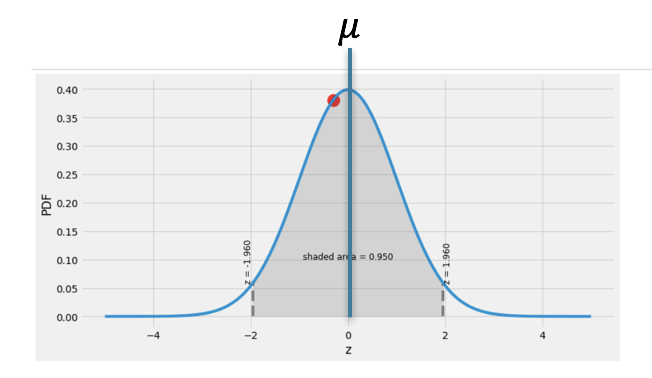
\includegraphics[width=\maxwidth{\textwidth}]{figures/normal_distribution.png}
    \caption{Error functions were evaluated with the assistance of a library: \emph{NeuronUnit} 
    were based on finding a normal distribution on electro physiology measurements, 
    and then measuring model outputs and mapping the model behavior onto
     a place on the experimental normal distribution. Scores that where closer to the
      experimental mean where deemed to be low in error.
	Z-scores obtained via NeuronUnit can be thought of as  }
	\label{figure\arabic{figurecounter}}
	
\caption{Caption}
	
\end{figure}
